\chapter{Background Estimation}\label{chapter:bkg}
%Monte Carlo simulated samples are used to model the signal and background processes expected to be observed in the proton-proton collision data used.
%
%
%
%all the effects observed in 
%
%Typically, most of the discrepancies observed can be accounted for by applying various corrective scale factors.
%Where a particular process is poorly described and/or lacking sufficient statistics in the signal region, data-driven estimates of the background are used to model ...

\section{Data and Simulation Samples}\label{sec:samples}
Out of the 37.8\fbinv of the proton-proton collision data at $\sqrt{s} = 13\TeV$ collected by CMS during 2016, 35.8\fbinv was certified by the collaboration as ``good'' to be used for physics analysis.

The difference between the certified value and the total data recorded is the result of various factors such as the unavailability of a detector.
Due to the prescaling of the electron triggers during the start of the most luminous runs, as discussed in Chapter~\ref{sec:triggerStrategy}, the ee channel uses a reduced dataset of 35.6\fbinv where none of the triggers considered were prescaled.
Events in the double lepton and single lepton datasets from across these ``good'' data runs are considered where the double and single lepton triggers respectively have fired, using the strategy described in Chapter~\ref{sec:triggerStrategy}.

The MC samples used to model signal and background processes that were considered are listed in table~\ref{tab:mcList}, which includes information on the number of events generated, their cross sections and the order in perturbative accuracy in QCD to which the generators calculated the processes.
For all the MC samples considered, the hadronisation of all the MC samples considered was undertaken using PYTHIA 8.
The NNPDF3.0 family of PDF sets was used as input for the generators of the MC samples, where the corresponding PDF sets were used depending on whether the sample was produced at LO or NLO and used either the four or five flavour scheme.

\begin{table}[htbp]
\topcaption {
The MC processes and their associated total number of events, cross sections and generators (and order in perturbative QCD accuracy they are calculated to), considered for the search for tZq in the dilepton final state. Both generators considered for the Z+jet background are also listed below.
}
\label{tab:mcList}
  \centering
  \resizebox{\textwidth}{!}{
% This right-aligns numbers in column, but centers them under column title.
 \begin{tabular}{cccc}
   \hline
   \textbf{MC process} & \textbf{Events} & \textbf{Cross section (pb)} & \textbf{Generator (Order)}   \\
   \hline
   tZq  & 14.5M & 0.0758  & aMC@NLO (NLO) \\
   \hline
   tHq  & 3.5M & 0.07462  & Madgraph (LO) \\
   \hline
   tWZ/tWll  & 50K & 0.01104  & Madgraph (LO) \\
   \hline
   t tW-channel & 7M & 35.85 & POWHEG (NLO) \\
   $\overline{\text{t}}$ tW-channel & 6.9M & 35.85 & POWHEG (NLO) \\
   \hline
   t s-channel & 2.9M & 10.32 & aMC@NLO (NLO) \\
   \hline
   t t-channel & 67.2M & 136.02 & POWHEG (NLO) \\
   $\overline{\text{t}}$ t-channel & 38.8M & 80.95 & POWHEG (NLO) \\
   \hline
   \ttbar & 77.1M & 831.76 & POWHEG (NLO) \\
   \hline
   \ttbarZ $\rightarrow$ ll$\nu\nu$ & 13.9M & 0.2529   & aMC@NLO (NLO) \\
   \ttbarZ $\rightarrow$ qq & 749K & 0.5297   & aMC@NLO (NLO) \\
   \hline
   \ttbarW $\rightarrow$ l$\nu$ & 5.3M & 0.2001   & aMC@NLO (NLO) \\
   \ttbarW $\rightarrow$ qq & 833K & 0.405  & aMC@NLO (NLO) \\
   \hline
   \ttbarH $\rightarrow$ bb & 3.8M & 0.2942 & POWHEG (NLO) \\
           $\rightarrow$ non bb & 4.0M & 0.2123 & POWHEG (NLO) \\
   \hline
   W+jets & 24.1M & 61526.7 & aMC@NLO (NLO) \\
   \hline
   Z+jets ($m_{Z} \geq 50\GeVcc $ & 146M & 5765.4 & Madgraph (LO) \\
   Z+jets ($10 \GeVcc \leq m_{Z} < 50\GeVcc$ & 35.3M & 18610.0 & Madgraph (LO) \\
   \hline
   Z+jets ($m_{Z} \geq 50\GeVcc $ & 151M & 5765.4 & aMC@NLO (NLO) \\
   Z+jets ($10 \GeVcc \leq m_{Z} < 50\GeVcc$ & 106M & 18610.0 & aMC@NLO (NLO) \\
   \hline
   WW $\rightarrow$ l$\nu$qq & 9.0M & 49.997  & POWHEG (NLO) \\
      $\rightarrow$ ll$nu\nu$ & 2.0M & 12.178 & POWHEG (NLO) \\
   \hline
   WZ $\rightarrow$ l$\nu$qq & 24.2M & 10.73 & aMC@NLO (NLO) \\
      $\rightarrow$ llqq & 26.5M & 5.606 & aMC@NLO (NLO) \\
      $\rightarrow$ lll$\nu$ 1.9M & 5.26 & aMC@NLO (NLO) \\
   \hline
   ZZ $\rightarrow$ ll$\nu\nu$ & 8.8M & 0.5644 & POWHEG (NLO) \\
      $\rightarrow$ llqq & 15.3M & 3.222 & aMC@NLO (NLO) \\
      $\rightarrow$ llll & 10.7M & 1.204 & aMC@NLO (NLO) \\
   \hline
   WWW & 240K & 0.2086 & aMC@NLO (NLO) \\
   \hline
   WWZ & 250K & 0.1651 & aMC@NLO (NLO) \\
   \hline
   WZZ & 247K & 0.05565 & aMC@NLO (NLO) \\
   \hline
   ZZZ & 249K & 0.01398 & aMC@NLO (NLO) \\
   \hline
   
 \end{tabular}}
\end{table}

To determine the impact of a number of theoretical uncertainties for a number of processes, a several dedicated samples, listed in table~\ref{tab:theorySampleList}, were used.
These systematic uncertainties are discussed further in Chapter~\ref{sec:theorySysts}.

\begin{table}[htbp]
\topcaption {
The dedicated MC samples used to determine the impact of theoretical uncertainties, including the associated total number of events, cross sections and generators (and order in perturbative QCD accuracy they are calculated to), considered for the search for tZq in the dilepton final state.
}
\label{tab:theorySampleList}
  \centering
 \resizebox{\textwidth}{!}{
 \begin{tabular}{cccc}
   \hline
   \textbf{MC process} & \textbf{Events} & \textbf{Cross section (pb)} & \textbf{Generator (Order)}   \\
   \hline
   tZq scale up & 6.9M & 0.0758  & aMC@NLO (NLO) \\
   tZq scale down & 7.0M & 0.0758  & aMC@NLO (NLO) \\
   \hline
   t tW-channel scale up & 998K & 35.85 & POWHEG (NLO) \\
   t tW-channel scale down & 994K & 35.85 & POWHEG (NLO) \\
   $\overline{\text{t}}$ tW-channel scale down & 1.0M & 35.85 & POWHEG (NLO) \\
   $\overline{\text{t}}$ tW-channel scale down & 999K & 35.85 & POWHEG (NLO) \\
   \hline
   t t-channel scale up & 5.7M & 136.02 & POWHEG (NLO) \\
   t t-channel scale down & 5.9M & 136.02 & POWHEG (NLO) \\
   t t-channel matching up & 6.0M & 136.02 & POWHEG (NLO) \\
   t t-channel matching down & 6.0M & 136.02 & POWHEG (NLO) \\
   $\overline{\text{t}}$ t-channel scale up & 4.0M & 80.95 & POWHEG (NLO) \\
   $\overline{\text{t}}$ t-channel scale down & 3.9M & 80.95 & POWHEG (NLO) \\
   $\overline{\text{t}}$ t-channel matching up & 4.0M & 80.95 & POWHEG (NLO) \\
   $\overline{\text{t}}$ t-channel matching down & 4.0M & 80.95 & POWHEG (NLO) \\
   \hline
   \ttbar ISR up & 156.5M & 831.76 & POWHEG (NLO) \\
   \ttbar ISR down & 149.8M & 831.76 & POWHEG (NLO) \\
   \ttbar FSR up & 152.6M & 831.76 & POWHEG (NLO) \\
   \ttbar FSR down & 156.0M & 831.76 & POWHEG (NLO) \\
   \ttbar matching up & 58.9M & 831.76 & POWHEG (NLO) \\
   \ttbar matching down & 58.2M & 831.76 & POWHEG (NLO) \\
   \hline   
 \end{tabular}}
\end{table}

%%% Alt Z+jets 
%During the study of the poor agreement between simulation and data for the aMC@NLO Z+jets samples considered, a number of alternative 
%To determine the impact of a number of theoretical uncertainties for a number of processes, a several dedicated samples, listed in table~\ref{tab:zPlusSamples}, were used.
%These systematic uncertainties are discussed further in Chapter~\ref{sec:subsec:zPlusJetsEstimation}.
%
%\begin{table}[htbp]
%\topcaption {
%The dedicated MC samples used to determine the impact of theoretical uncertainties, including the associated total number of events, cross sections and generators (and order in perturbative QCD accuracy they are calculated to), considered for the search for tZq in the dilepton final state.
%}
%\label{tab:zPlusSamples}
%  \centering
% \resizebox{\textwidth}{!}{
% \begin{tabular}{cccc}
%   \hline
%   \textbf{MC process} & \textbf{Events} & \textbf{Cross section (pb)} & \textbf{Generator (Order)}   \\
%   \hline
%   tZq scale up & 6.9M & 0.0758  & aMC@NLO (NLO) \\
%   \hline   
% \end{tabular}}
%\end{table}
%
\section{Simulation Corrections}\label{sec:simCorrections}
Simulation is unable to fully recreate all the effects observed in data, either because certain parameters are not precisely known or cannot be calculated.
To account for these discrepancies, corrective scale factors are used to reweight MC on a per event basis.
Such scale factors are usually derived as a function of \pt and $\eta$ so as to account for the variation of the detector response in both.
These corrections are used to correct simulation for lepton identification, isolation and reconstruction efficiencies, b-tagging efficiencies, the poor modelling of pileup in simulation, and the detector resolutions observed in data.

\subsection{Miscalibrated Tracker APV}\label{subsec:hipEffect}
During the first half of data taking in 2016 the silicon strip detector suffered from instantaneous luminosity dependent  hit finding inefficiencies, particularly in high occupancy regions, due to saturation in the pre-amplifier in the front end electronics~\cite{Fiori:2016ebh}.
This issue was resolved by changing the configuration of the electronics.
While the affected part of the dataset has been reprocessed to mitigate the impact on the quality of the data taken, there is still a negative impact on the detector efficiency for objects that rely upon highly efficient tracking data.
This is accounted for by the weighting of events appropriately when the scale factors are produced, either centrally by CMS or those derived for the analysis (\ie the trigger scale factors), so that a single scale factor is applied to a simulated event.

%In most cases, centrally produced scale factors are derived for the whole of the 2016 dataset to account for this, but 
%for muons they were provided for both the affected and unaffected parts of the dataset separately.
%Consequently, the muon scale factors were weighted according to the luminosity they corresponded to before their application to simulation.
%Similarly, the muon trigger scale factors that were derived were also produced 

\subsection{Lepton Efficiency}\label{subsec:leptonRecoSFs}
The identification, isolation and reconstruction efficiencies of leptons are calculated using measurements of $Z \rightarrow l^{+} l ^{-}$ events with the \emph{tag-and-probe} method~\cite{CMS:2008rxa}.
Using events within a dilepton invariant mass window to ensure a high purity, from this large statistics lepton sample, the method ``tags'' and ``probes'' the leptons where one has passed a tight and the other a loose selection criteria.
For source of each efficiency and lepton flavour, the efficiency is given as the fraction of events where the probe leptons passed the relevant selection criteria.
This methodology is used to create corrective scale factors for each component and these are multiplicatively applied to each leptons' event weight as functions of their \pt, $\eta$, and flavour.


The efficiencies for the triggers used were calculated by considering events that pass triggers which are weakly correlated with the lepton triggers.
By counting these events and whether or not they pass or fail the analysis triggers, the trigger efficiency is estimated as follows:

\begin{equation}
\epsilon_{trigger} = \frac{N_{X triggers + lepton triggers}}{N_{X triggers}} \\
\end{equation}

where $N_{X trigger}$ is the number of events which have passed the lepton selection criteria and the cross triggers, and $N_{X triggers + lepton triggers}$ is $N_{X trigger}$ and the number of events which have also passed the lepton triggers.

As the trigger requirements are applied to both simulated and data events, a scale factor of the ratio of the trigger efficiency in data and in simulation is applied to the event weight in simulation.

\editComment{The following below is to be updated ASAP. Muon POG has found that the muon tracking SFs are no longer necessary - were the result of buggy derivation. Also, the dimuon trigger DZ leg is known to be heavily impacted by the HIP issue, but the non-DZ leg (available Runs B-G) was fine but not mentioned in the TOP Trigger twiki despite others using it and maintaining a high dimuon trigger efficiency.
Initial tests reveal that \pT and $\eta$ binned SFs for $\mu\mu$ may not be required... Will result in smaller statistical uncerts.
Unlikely to have time to resolve before submission -> something for Corin and Kate to look at!
}

For the scale factors derived for the ee and e$\mu$ channels, a constant scale factor was found to be sufficient to account for the differences between data and simulation.
In the case of the $\mu\mu$ channel however, the scale factor was produced as a function of both \pt and $\eta$ due to the inefficiencies observed for the double muon triggers with $d_{Z}$ cuts caused by the miscalibrated tracker APV (discussed in Chapter~\ref{subsec:hipEffect}.
As the equivalent double muon triggers without the $d_{Z}$ cuts were pre-scaled during runs with high instantaneous luminosity, these triggers were not considered.

\subsection{Lepton Energy Corrections}\label{subsec:leptonEnergyCorrections}
\subsubsection{Electron Regression and Energy Scale and Smearing Corrections}
Two types of energy corrections which have been produced by the CMS EGM POG are applied to electrons and photons, energy regression and energy scale and smearing corrections.
These corrections are applied to both MC simulation and data and are used to improve the electron resolution obtained and to resolve the observed discrepancies between them.

Using simulation for tuning, energy regression obtains the best possible energy resolution by using the detector information to correct the reconstructed object energy.
The disagreement between data and MC is resolved by scaling the data energy to the MC energy scale and smearing the MC so that it has the same energy resolution as data. 

These corrections are pre-applied onto the PF electron collections used.

\subsubsection{Rochester Corrections}
The muon momentum scale and resolution correction methods developed by the University of Rochester~\cite{rochester}, known as \emph{Rochester Corrections}, are used to remove any muon momentum bias from any detector misalignment, reconstruction or uncertainties in the magnetic field for both MC and data.
These corrections are derived with high \pt ($> 20\GeVc$) muons from Z $ \rightarrow \mu\mu$ decays using a two step method, where the muons are binned in charge, $\eta$ and $\phi$.
The first step requires the mean inverse transverse momenta of the muons reconstructed from data and simulation to be the same as the corresponding values from a perfectly aligned detector.
These corrections are tuned in the second step by using the $M_{\mu^{+1}\mu^{-1}}$ peak for a perfectly aligned detector to calibrate the corrections.
This removes any sensitivity to detector efficiencies or physics modelling.

The Rochester Corrections are applied to each muon an event weight that is a function of the muon's charge, \pt, $\eta$ and $phi$.

\subsection{Jet Energy Corrections}\label{subsec:jesjer}
As described in Chapter~\ref{subsubsec:JECs}, the JECs are applied to account for the non-uniform response in \pT and $eta$ of the detector by comparing the differences between the generator level and detector level responses.

In addition to these corrections, as the Jet Energy Resolution (JER) observed in data is approximately 10\% poorer than that in observed simulation, the 4-vectors of simulated jets are smeared as functions of generator level and reconstructed \pt and $\eta$ to account for this~\cite{Khachatryan:2016kdb}.

\subsection{b-tagging Efficiency}\label{subsec:btagEff}
The B-Tag and Vertexing (BTV) Physics Object Group measures the b-tagging efficiency and misidentification rates for b and light flavoured jets in data and MC simulation (multijet and \ttbar) of the algorithms which they support~\cite{Sirunyan:2017ezt}.
From these measurements b-tagging efficiency scale factors are produced and provided for analysts to apply to simulated events to correct differences observed between data and simulation.
These scale factors, as functions of the jet flavour, \pT and $\eta$, are used to alter the weight of the selected MC events.
This methodology was chosen as it involves only changing the weight of the selected MC events which, unlike other methods, avoids events migrating into different b-tag multiplicity bins and having events with potentially undefined variables such as the top mass.

\subsection{\PU Modelling}\label{subsec:puSF}
It is challenging to model variations in the number of \PU interactions that result from the changing LHC conditions.
Therefore MC events are reweighted as a function of the number of primary vertices so that the simulated PU interactions resemble what is observed in data.

The \PU SF is determined as a function of the number of primary vertices, $n_{PV}$, present by comparing $n_{PV}$ in minimum bias data over the running period considered to $n_{PV}$ for simulated events.

\subsection{Top quark \pt}
A scale factor is applied to \ttbar MC as a function of the top's and anti-top's generator level transverse momenta to account for the \pt spectra of top quarks in data being significantly softer than that predicted by LO and NLO precision MC simulation~\cite{Khachatryan:2015oqa}.


\section{Signal Region Simulated Backgrounds}\label{sec:simBackgrounds}
The impact of the application of the full event selection and simulation corrections in the signal region on the simulated samples, including non-prompt lepton contribution estimated from data, compared to data is shown in table~\ref{tab:signalYields}.

While jet cleaning and tight isolation criteria for leptons has significantly reduced the non-prompt lepton contributions, completely removing the W+jets process, the signal region is still dominated by a number of background processes.
The two dominant background processes are Z+jets and \ttbar, with contributions of a similar order to tZq from the single top tW-channel, \ttbarZ, WZ and ZZ processes.
The remaining single top (tHq, tWZ, s-channel, t-channel), \ttbarW, \ttbarH, WW and triboson backgrounds produce contributions smaller than the signal process.

\begin{table}[htbp]
\topcaption{The number of observed events in data, the data-driven estimate of the non-prompt leptons and the number of expected events in simulation in the signal region fllowing the full event selection for each of the separate channels and with both channels combined. The aMC@NLO sample is used for the Z+jets contriubtion given 
}\label{tab:signalYields}
\centering
\begin{tabular}{lccccc}
\hline
Channel &  $ee$ & $\mu\mu$ & Combined \\
\hline
Signal (SM tZq) & 30.242 &  54.508 & 84.750     \\
Backgrounds: & & & \\
tWZ\@: & 6.439 & 10.779 & 17.218    \\
tHq: & 0.173 & 0.372 & 0.545    \\
ttW\@: & 7.249 & 10.681 & 17.930    \\
ttZ\@: & 61.882 & 110.471 & 172.353    \\
ttH\@: & 4.916 & 9.554 & 14.470    \\
\ttbar: & 1653.457 & 3219.360 & 482.817    \\
tW\@: & 95.989 & 177.527 & 273.516    \\
s-channel: & 0.000 & 0.000 & 0.000    \\
t-channel: & 0.612 & 0.995 & 1.607    \\
WW\@: & 1.339 & 2.4475 & 3.786    \\
WZ\@: & 73.466 & 126.656 & 200.122    \\
ZZ\@: & 51.827 & 92.980 & 144.807    \\
WWW\@: & 0.114 & 0.305 & 0.419    \\
WWZ\@: & 1.327 & 2.207 & 3.534    \\
WZZ\@: & 1.540 & 2.470 & 4.010    \\
ZZZ\@: & 0.661 & 1.087 & 1.748    \\
W + jets: & 0.000 & 0.000 & 0.000    \\
Z + jets: & 3293.634 & 6245.353 & 9538.987    \\
\hline
NPLs: & 37.787 & 30.889 & 68.676   \\
\hline
Data & 5284 & 9665 & 14949    \\
Total MC & 5284.867 & 10067.752 & 15352.619    \\
Total MC + NPLs & 5322.654 & 10098.641 & 15361.377    \\
\hline
\end{tabular}
\end{table}

\section{Data-driven Background Estimation}\label{sec:dataDrivenBackground}

\subsection{Non-Prompt Leptons}\label{sec:NPLs}
Leptons which are produced from events where at least one jet is incorrectly reconstructed as a lepton (predominately electrons) or a lepton from the decay of heavy quarks (predominately muons) are known as \emph{non-prompt leptons} (NPLs).
The majority of these events are produced by \ttbar decaying semi-leptonically and W+jets, with smaller contributions from QCD and single top production.
Given the difficulty in accurately modelling QCD processes and the very low statistics of such processes passing the lepton selection and isolation criteria could result in an inaccurate estimate of such processes from simulation alone, the NPL contribution is estimated with data.

This data-driven estimation is based off the methodology used in top quark pair production~\cite{CMS:2016syx} and same charge SUSY searches~\cite{CMS:2015vqc}.
This approach takes advantage of the fact that the vast majority of the event yields for same charge lepton pairs result from non-prompt and charge misidentified leptons, with some contributions from prompt leptons (such as \ttV).
As these backgrounds are independent of the charge of the lepton pairs, it is expected that the nominal opposite charge event selection would have a similar contribution.

Therefore by inverting the signal region's oppositely charged lepton requirement (\ie the leptons must have the same charge), a same charge control region can be defined which is dominated by NPL events while containing some contributions from prompt lepton events, charge misidentification and real same charge pairs.

Using this control region, a data-driven estimate of the contribution of opposite charge NPLs can be derived using Equation~\ref{eq:NPL}:

\begin{equation}\label{eq:NPL}
 N_{data}^{OS non-prompt} = (N_{data}^{SS} - N^{SS}_{real + mis-ID}).\frac{N_{MC}^{OS non-prompt}}{N_{MC}^{SS non-prompt}}
\end{equation}

where $N_{data}^{SS}$ is the total number of same charge events observed in data and $N^{SS}_{real + mis-ID}$ is the expected number of real same charge events and events with charge misidentification.

The ratio of opposite charge and same charge NPLs in simulation, $N_{MC}^{OS non-prompt}$ and $N_{MC}^{SS non-prompt}$, is used to appropriately normalise this estimate and uses the generator level information to correctly identify how the leptons were produced.
The W+jets, \ttZ, \ttW, and single top simulated samples which have sufficient statistics in the control region are used to calculate this ratio as these processes are expected to be the predominant source of non-prompt leptons for this analysis.

The event yields of the simulated samples and data following the full event selection in the same lepton charge control region, the same sign background contributions not accounted for by simulation, ratio of same charge to opposite charge event yields and the data-driven NPL contribution estimate are given in table~\ref{tab:fakeLeptonYields}.

%\editComment{Add bit about study into number of expected SS events with no fakes from DY mis-ID. Found to be negligible for mumu and < 1\% for ee - should be well covered by syst}

\begin{table}[htbp]
\topcaption{The event yields following the full event selection ratio of same to opposite charge lepton events, the same sign background contributions not accounted for by simulation, ratio of same charge to opposite charge event yields and the estimated non-prompt lepton contribution following all selection cuts.
\editComment{TODO: Add uncerts and e$mu$ values}
}
\centering
\begin{tabular}{l | ccccc}
\hline
Source &  $ee$ & $\mu\mu$ & $e\mu$ \\ 
\hline
\ttbar (SS): & 30.971 & 71.539 & e  \\
\ttV (SS): & 6.729 & 10.479 & e  \\ 
Single Top (SS): & 1.764 & 2.624 & e  \\
W + jets (SS): & 0.0 & c & e  \\
Z + jets (SS): & 44.400 & 0.0 & 1.378  \\
VV (SS): & 2.148 & 0.348 & e \\
VVV (SS): & -0.024 & 0.098 & e \\
\hline
Total background (SS): & 85.988 & 85.088 & e \\ 
Data: & 126.0 & 125.0 & e  \\ 
\hline
SS data (bkg): & 40.012 & 39.912 & e\\
\hline
Non W/Z (SS): & 1.681 & 2.613 & e\\
Non W/Z (OS): & 1.579 & 2.337 & e\\
R (OS/SS): & 0.939 & 0.894 & e\\
\hline
NPL estimate: & 37.571 & 35.681 & e\\
\hline
\end{tabular}
\label{tab:fakeLeptonYields}
\end{table}

\subsection{Z+jets Background}\label{subsec:zPlusJetsEstimation}
Following the application of the full event selection and simulation corrections in the signal region both the Madgraph (LO) and aMC@NLO (NLO) Z+jets samples listed in table~\ref{tab:mcList} were compared.

In contrast to the correct normalisation of Madgraph Z+jets samples that was seen in the signal region and both of the Z+jets control regions, it was observed that there was a dramatic normalisation offset for the aMC@NLO Z+jets samples.

Figures~\ref{},~\ref{},~\ref{},~\ref{} and ~\ref{} show that that despite this scaling issue, the aMC@NLO Z+jets samples did better describe the higher jet multiplicities and the kinematics of the four leading jets in the nominal Z+jets control region defined in Chapter~\ref{subsec:zPlusJetsCR}.

\editComment{Update plots so that the colour used, labels, and legend are clearer. Consider using log plots for more detail?}
\editComment{Also cmbine plots for both channels - currently only have separate channels to hand}

\begin{figure}[tbp]
\centering
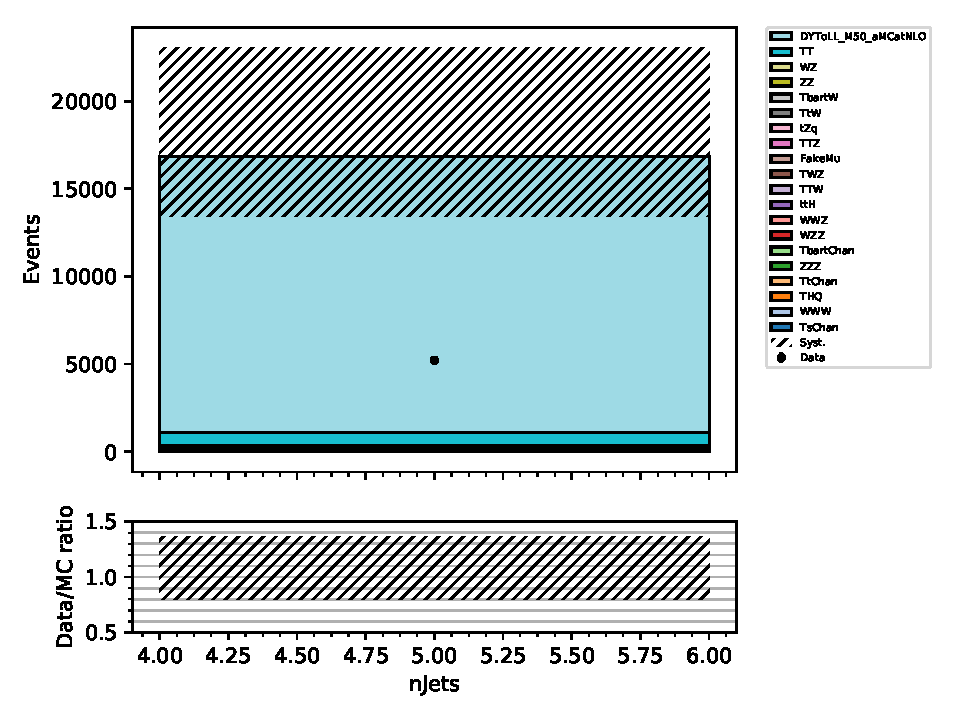
\includegraphics[width=0.47\textwidth]{figs/tzq-fullSelection-plots/plots_ee_zPlus/nJets.pdf}
\caption{
The distributions of the number of jets in the nominal Z+jets control region following the application of the full control region event selection and simulation corrections for the combination of both channels.
}
\label{fig:zPlusCR_nJets}
\end{figure}

\begin{figure}[tbp]
\centering
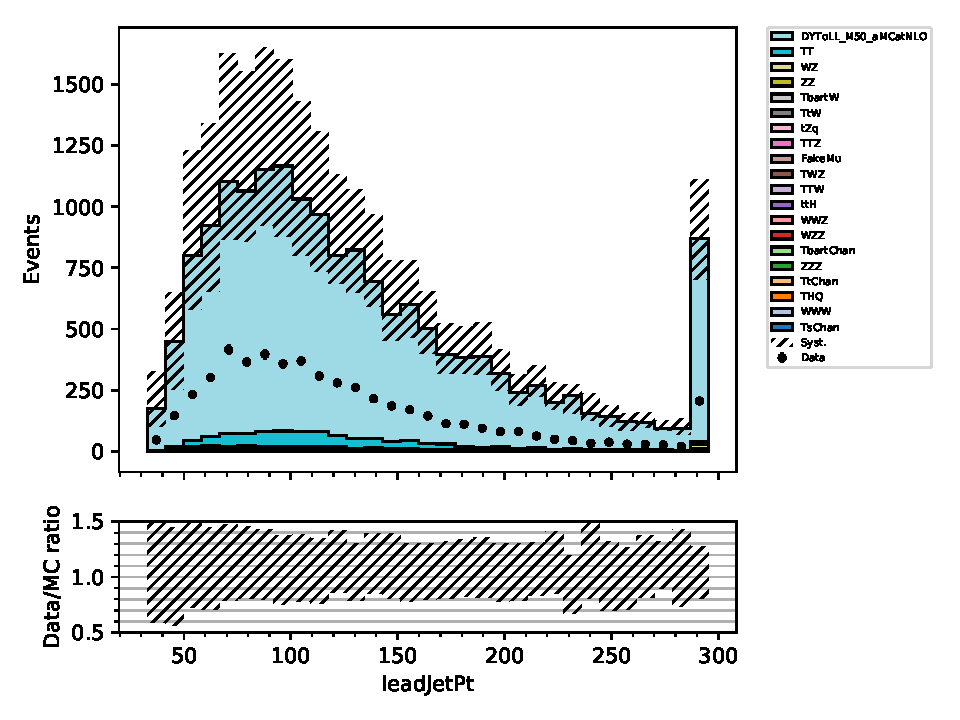
\includegraphics[width=0.47\textwidth]{figs/tzq-fullSelection-plots/plots_ee_zPlus/leadJetPt.pdf}
\caption{
The distributions of the leading jet \pt in the nominal Z+jets control region following the application of the full control region event selection and simulation corrections for the combination of both channels.
}
\label{fig:zPlusCR_leadJetPt}
\end{figure}

\begin{figure}[tbp]
\centering
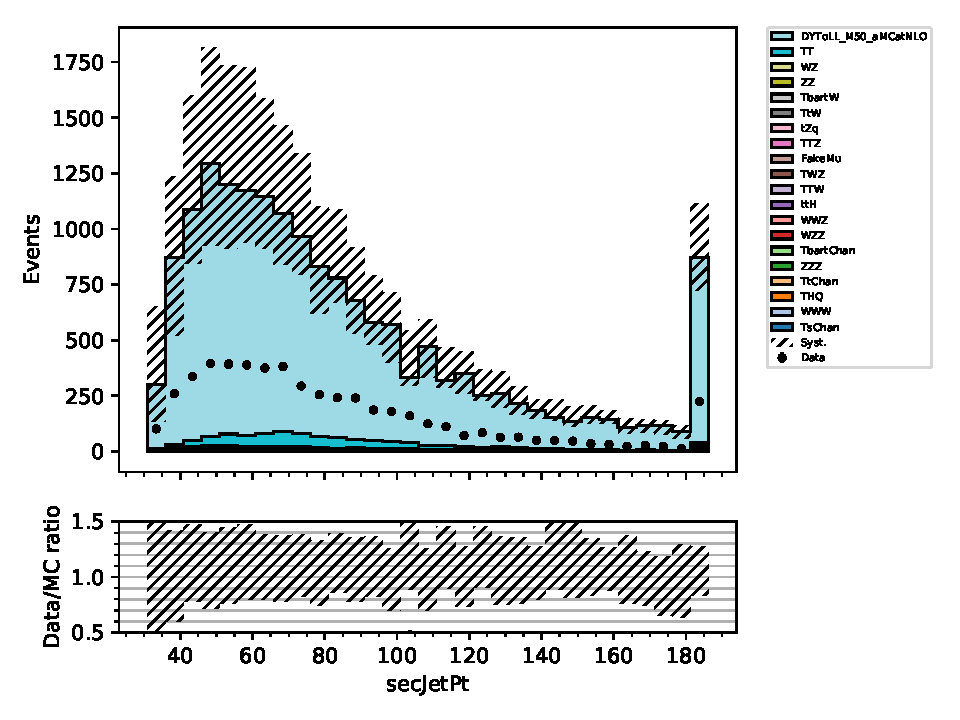
\includegraphics[width=0.47\textwidth]{figs/tzq-fullSelection-plots/plots_ee_zPlus/secJetPt.pdf}
\caption{
The distributions of the subleading jet \pt in the nominal Z+jets control region following the application of the full control region event selection and simulation corrections for the combination of both channels.
}
\label{fig:zPlusCR_secJetPt}
\end{figure}

\begin{figure}[tbp]
\centering
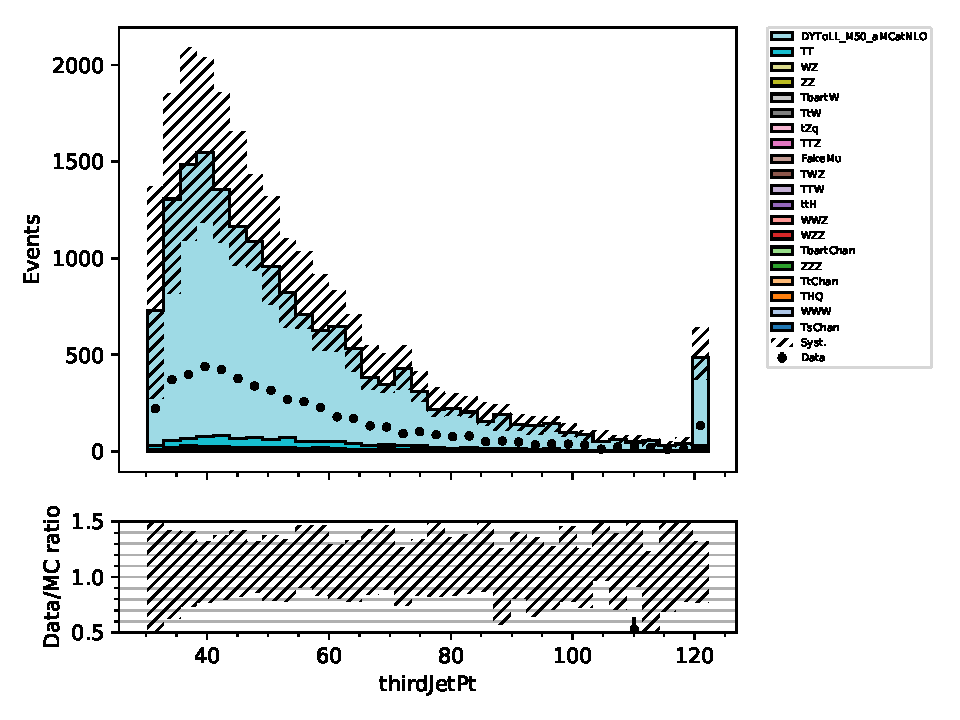
\includegraphics[width=0.47\textwidth]{figs/tzq-fullSelection-plots/plots_ee_zPlus/thirdJetPt.pdf}
\caption{
The distributions of the third jet \pt in the nominal Z+jets control region following the application of the full control region event selection and simulation corrections for the combination of both channels.
}
\label{fig:zPlusCR_thirdJetPt}
\end{figure}

\begin{figure}[tbp]
\centering
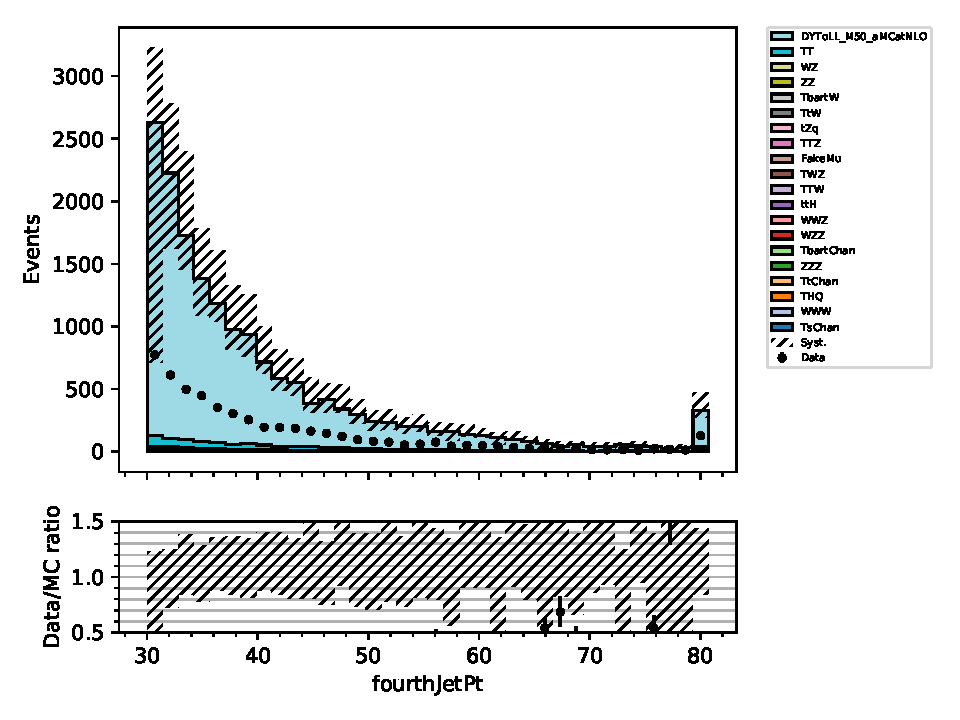
\includegraphics[width=0.47\textwidth]{figs/tzq-fullSelection-plots/plots_ee_zPlus/fourthJetPt.pdf}
\caption{
The distributions of the fourth jet \pt in the nominal Z+jets control region following the application of the full control region event selection and simulation corrections for the combination of both channels.
}
\label{fig:zPlusCR_fourthJetPt}
\end{figure}

Following observing this normalisation offset, a number of alternative Z+jets samples which were binned as a function of the Z boson's \pT and the number of jets produced by the hard process were also considered.
In contrast to the nominal Z boson mass binned samples, the alternative Z+jets samples generated by Madgraph and aMC@NLO were found to poorly describe the shapes of Z boson and jet distributions.
Consequently, these alternative samples were not considered as viable replacements of the Z boson mass binned Z+jets samples.

As having a NLO description of this large multi-jet background was highly desirable in light of the event selection requirements, it was decided to use nominal Z+jets control region to determine the correct normalisation of the aMC@NLO Z+jets samples.
The details of how this normalisation was achieved using the statistical analysis tool that was used to produce the analysis' results is described in Chapter~\ref{subsec:combineNormalisation}.

\subsection{\ttbar Background}\label{subsec:ttbarEstimation}
The \ttbar enriched control region, as defined in Chapter~\ref{subsec:ttbarCR}, was designed to provide an orthogonal region which was topologically similar to the signal region in order to validate:
\begin{itemize}
\item whether or not the simulated \ttbar sample used accurately modelled the \ttbar process;
\item and if not, to be used to derive a data-driven estimate for \ttbar.
\end{itemize}

As good agreement was observed between data and MC simulation for both the overall normalisation and the shapes of individual variables, it was determined that a data-driven estimate of the \ttbar contribution was unnecessary.

Examples of this good agreement between simulation and data for the number of jets, number of b-tagged jets, jet \pT for the leading four jets, invariant mass of the W boson ``candidate'', the leptons' \pt and invariant mass and \pt are given in figures~\ref{fig:ttbarCR_nJets},~\ref{fig:ttbarCR_jetPt}, and~\ref{fig:ttbarCR_leptons}.

\editComment{Update plots so that the colour used, labels, and legend are clearer. Consider using log plots for more detail?}

\begin{figure}[tbp]
\centering
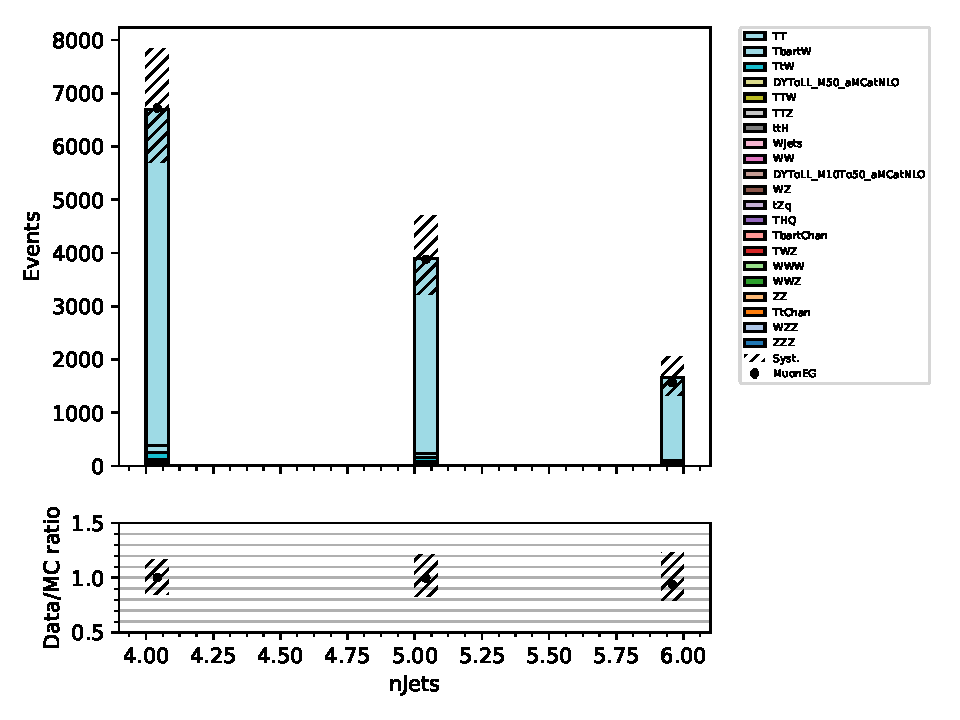
\includegraphics[width=0.47\textwidth]{figs/tzq-fullSelection-plots/plots_emu/nJets.pdf}
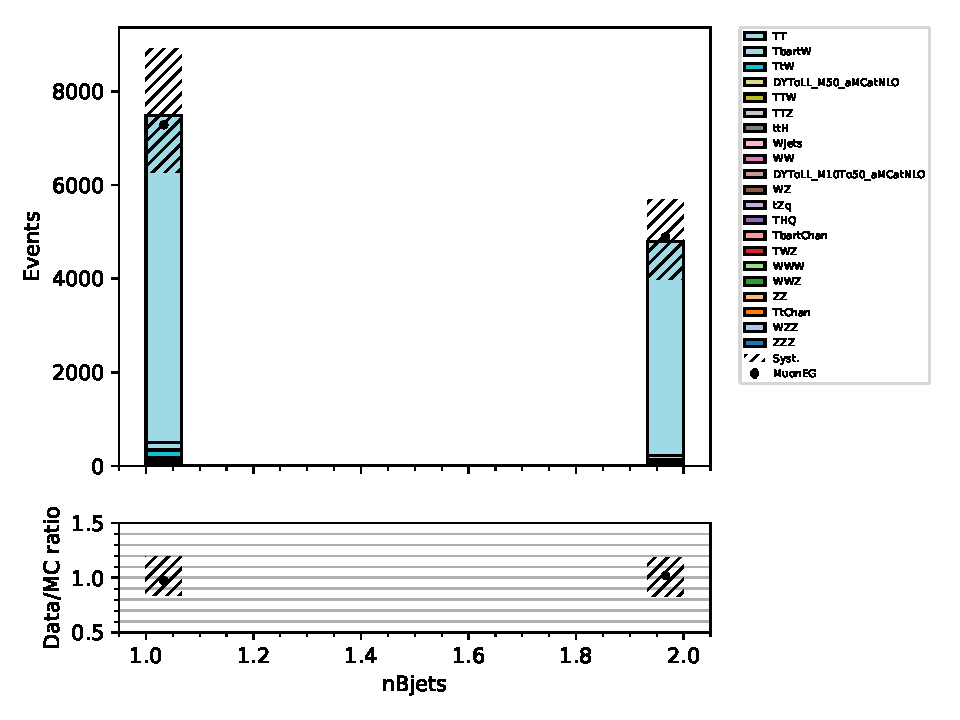
\includegraphics[width=0.47\textwidth]{figs/tzq-fullSelection-plots/plots_emu/nBjets.pdf}
\caption{
The distributions of the number of jets and the number b-tagged jets for the \ttbar control region following the application of the full control region event selection and simulation corrections.
}
\label{fig:ttbarCR_nJets}
\end{figure}

\begin{figure}[tbp]
\centering
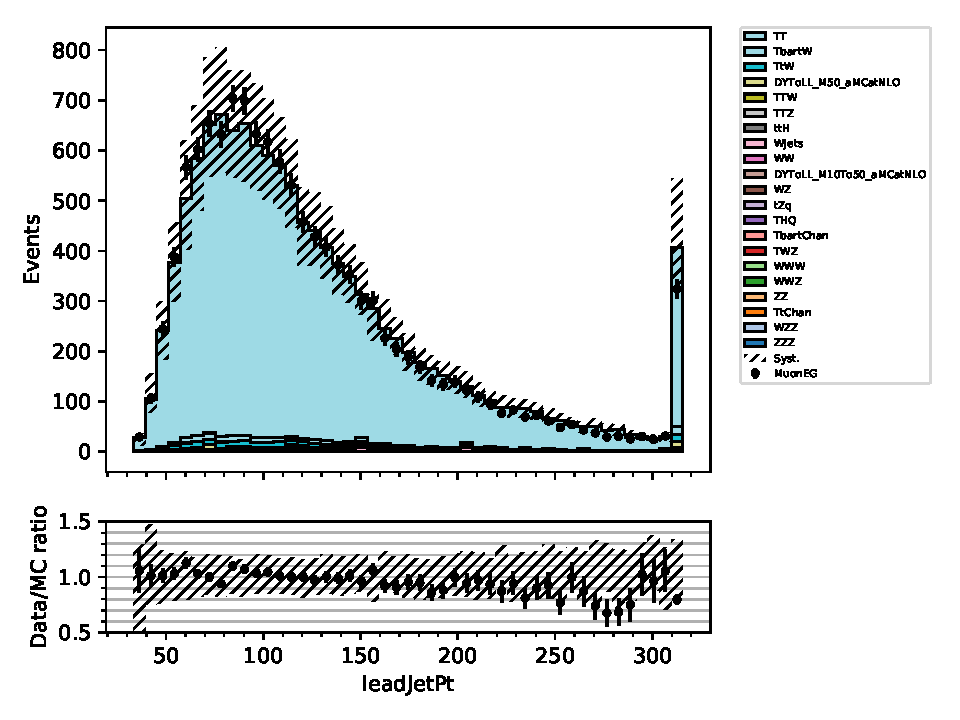
\includegraphics[width=0.47\textwidth]{figs/tzq-fullSelection-plots/plots_emu/leadJetPt.pdf}
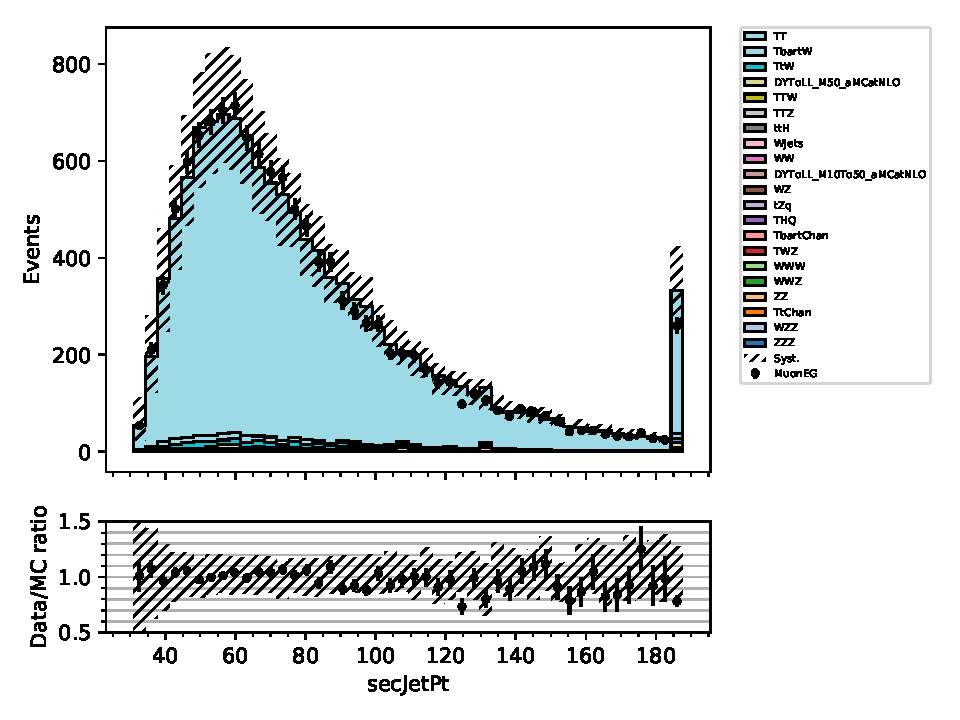
\includegraphics[width=0.47\textwidth]{figs/tzq-fullSelection-plots/plots_emu/secJetPt.pdf}
\\
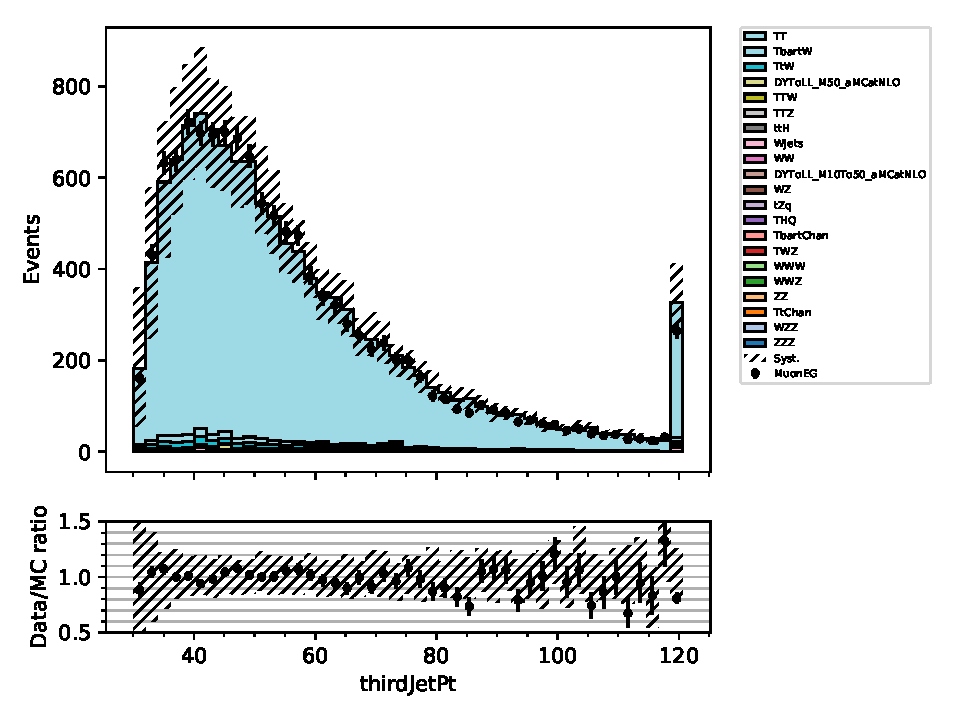
\includegraphics[width=0.47\textwidth]{figs/tzq-fullSelection-plots/plots_emu/thirdJetPt.pdf}
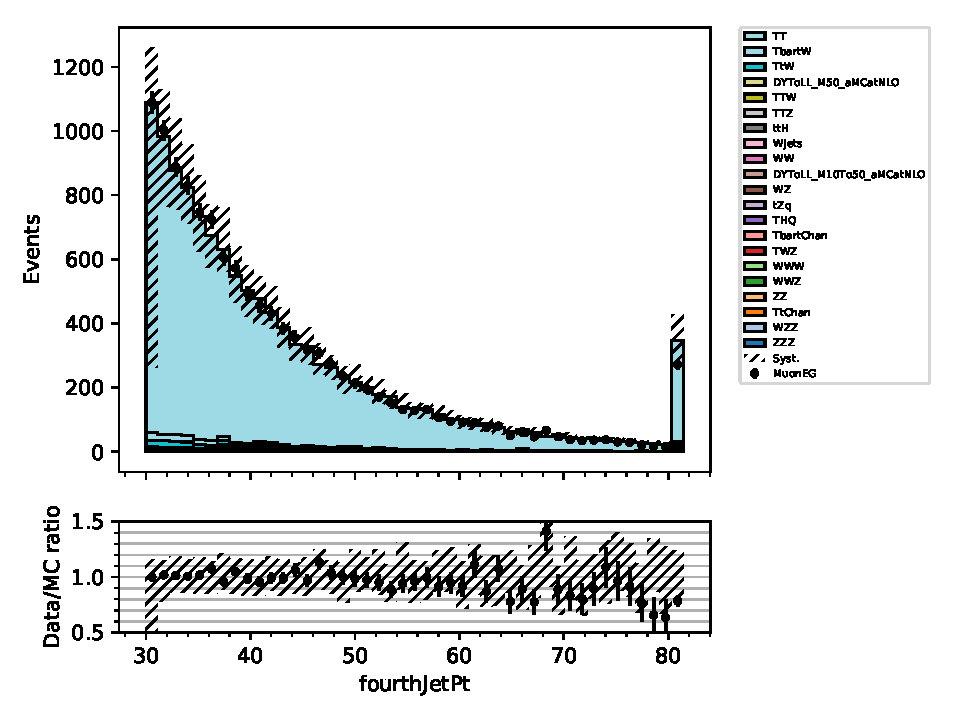
\includegraphics[width=0.47\textwidth]{figs/tzq-fullSelection-plots/plots_emu/fourthJetPt.pdf}
\caption{
The distribution of the \pt of the four leading jets for the \ttbar control region following the application of the full control region event selection and simulation corrections.
}
\label{fig:ttbarCR_jetPt}
\end{figure}

\begin{figure}[tbp]
\centering
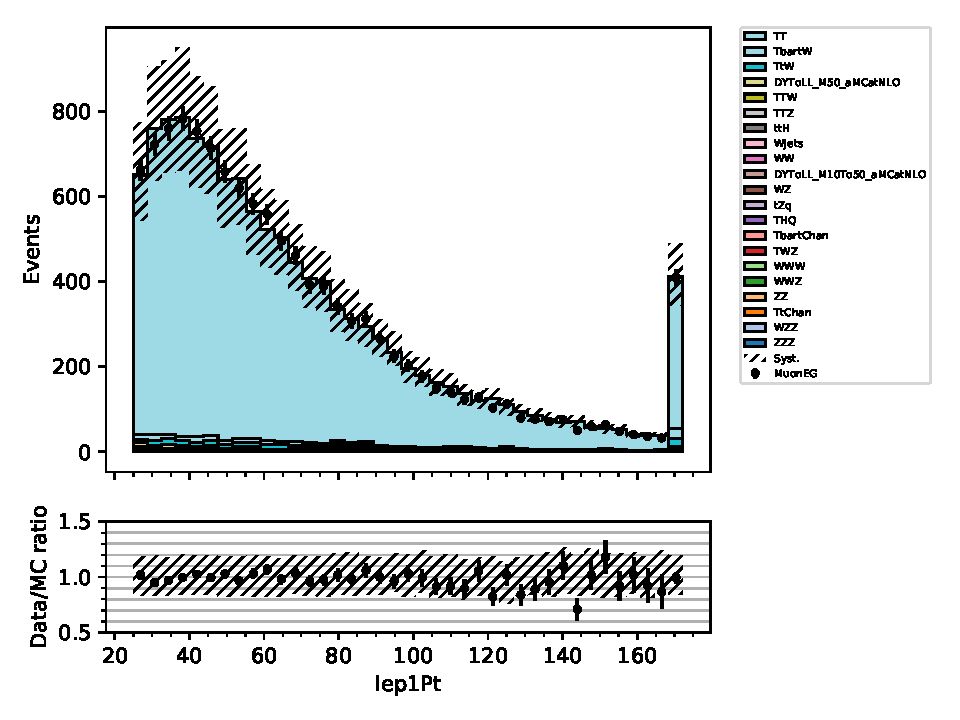
\includegraphics[width=0.47\textwidth]{figs/tzq-fullSelection-plots/plots_emu/lep1Pt.pdf}
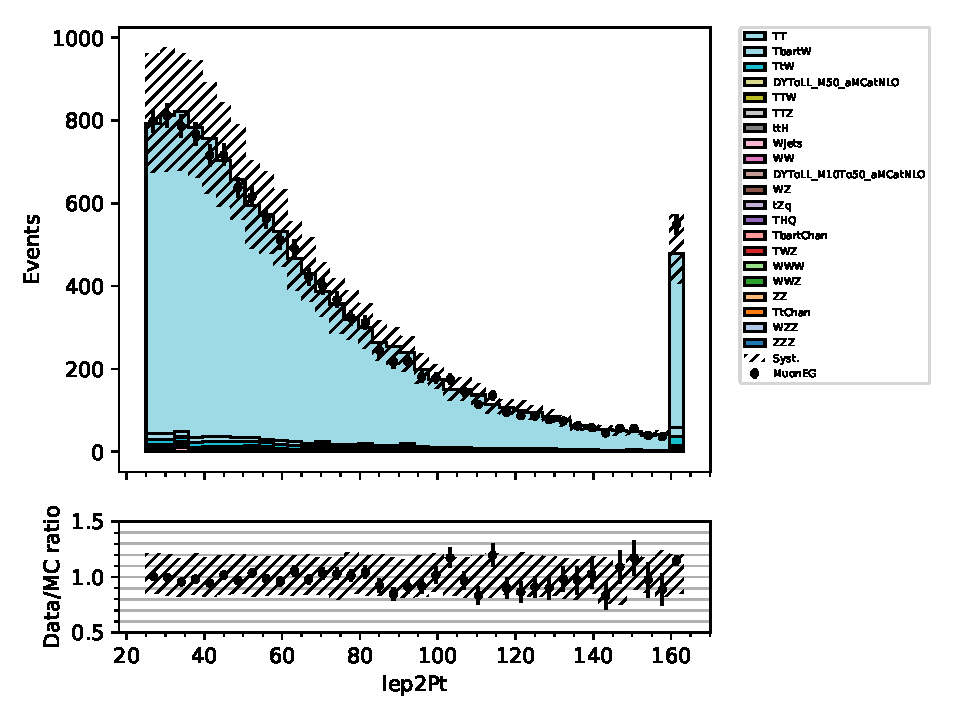
\includegraphics[width=0.47\textwidth]{figs/tzq-fullSelection-plots/plots_emu/lep2Pt.pdf}
\\
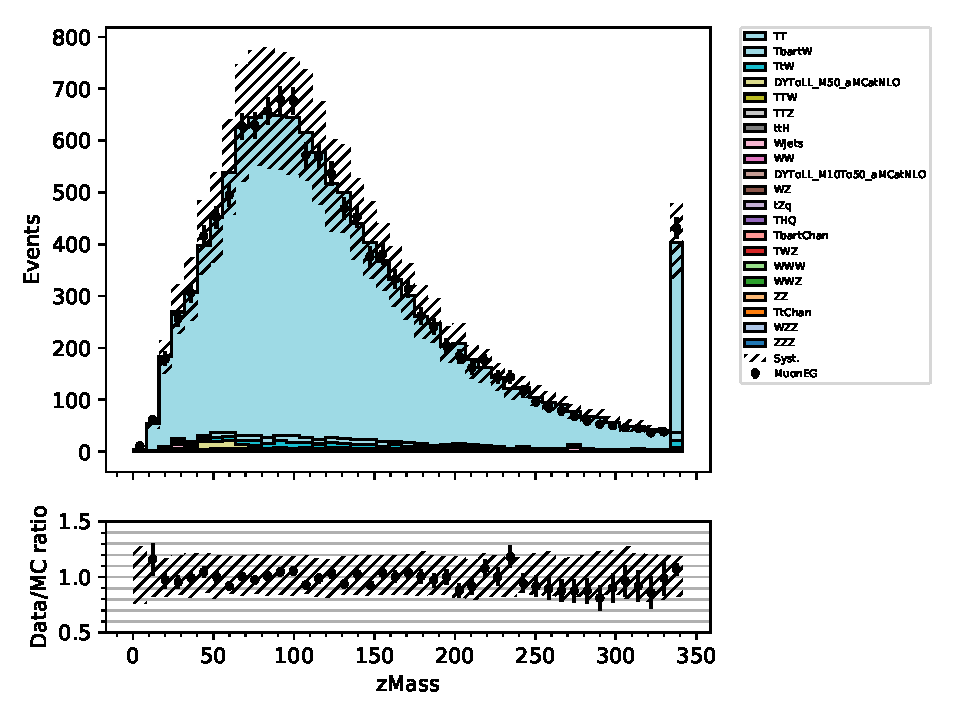
\includegraphics[width=0.47\textwidth]{figs/tzq-fullSelection-plots/plots_emu/zMass.pdf}
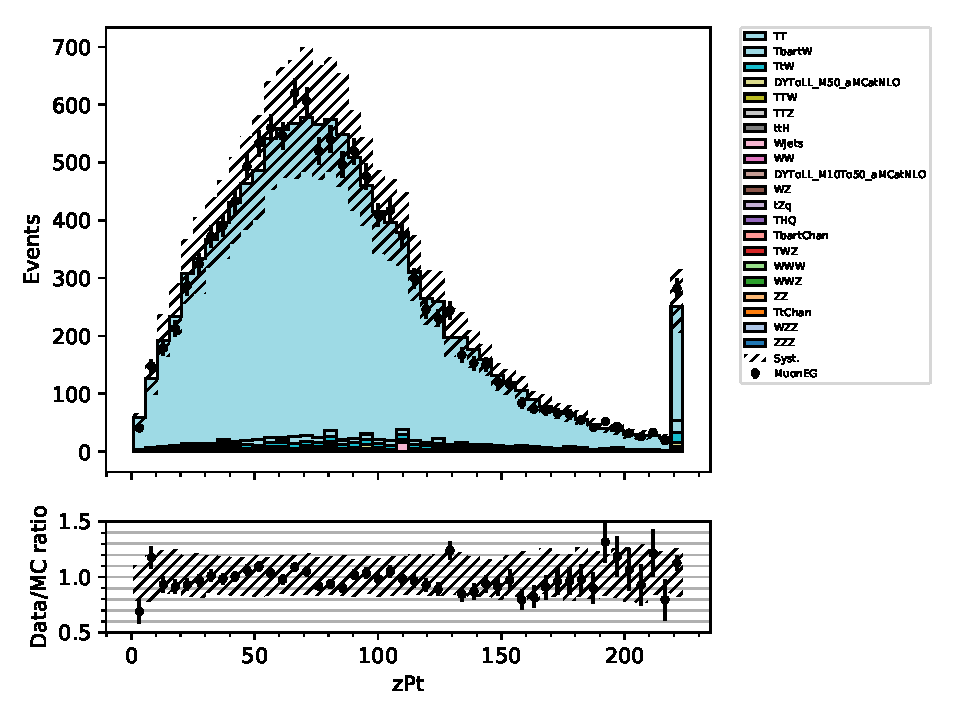
\includegraphics[width=0.47\textwidth]{figs/tzq-fullSelection-plots/plots_emu/zPt.pdf}
\caption{
The distribution of the selected electron and muon \pT and their combined invariant mass and \pt for the \ttbar control region following the application of the full control region event selection and simulation corrections.
}
\label{fig:ttbarCR_leptons}
\end{figure}

\section{Multivariate Analysis Techniques}\label{sec:mvas}
Multivariate Analysis (MVA) techniques are commonly used to further enhance the separation between signal and background processes given the difficulty in identifying rare or background dominated processes through the sole use of individual cuts.

Therefore, given the small cross section and topology of the dilepton final state of tZq, a MVA method was used to enhance the separation between the signal and background following the application of the selection cuts described in Chapter~\ref{chapter:tzq-search}.
The \emph{Boosted Decision Tree}~(BDT) MVA technique was chosen as it a widely used and supported technique which those undertaking this analysis were familiar with.

\subsection{Boosted Decision Trees}\label{subsec:bdt}
Figure~\ref{fig:decisionTree} illustrates a simple decision tree, where a series of sequential binary decisions (nodes) are made on a single input variable (\emph{feature}), $x_{i}$, until a leaf node is reached and the object is classified as either signal or background.

\begin{figure}[htb]
\centering
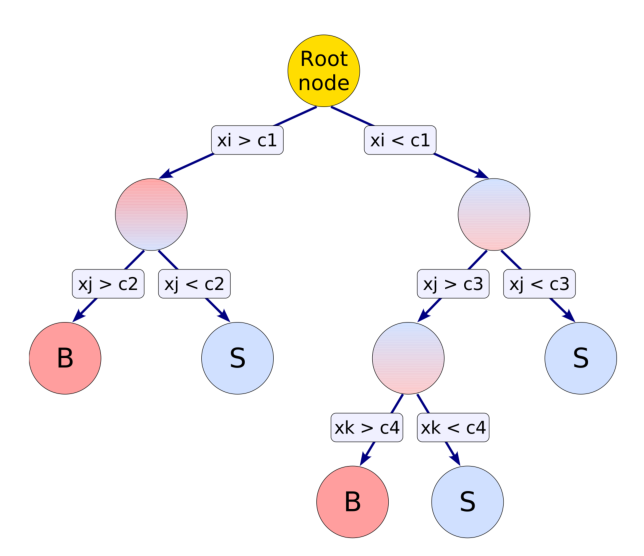
\includegraphics[width=0.97\textwidth]{figs/background-estimation/decisionTree.pdf}
\caption{A simple decision tree where repeated cuts on the variables $x_{i}$ are perfomed until a leaf node is reached and the object is classified as either signal or background~\cite{Hocker:2007ht}.
}
\label{fig:decisionTree}
\end{figure}

As the decision criteria for each node is dependent on the decisions of the preceding notes, decision trees have the potential to obtain better separation between signal and background processes through individual cuts on isolated variables.

Without any prior knowledge of the system however, a single isolated tree is not expected to be an efficient classifier.
Despite this however, such a weak learner will still contain some knowledge about the underlying structure of the classification problem.
\emph{Boosting} aims to exploit this knowledge by using an ensemble of repeatedly trained weak learners to produce a more effective classifier.
Following each training iteration the dataset is reweighted based on the success of the previous classifiers in order to force the weak learners to attempt to classify harder to identify objects.
At the end of this process a weighted average (based) of all the weak learners are combined to produce a single strong learner.

\emph{Bagging} is a similar concept to boosting, but involves each weak learner being trained on a random subset of the training sample, where every element has an equal probability of being sampled, rather than the whole training sample.

Therefore by extending boosting (or bagging) to decision trees, the resultant forest of \emph{Boosted Decision Trees} produces a classier that is both much more effective and resilient to fluctuations in the training sample than one created by a single tree.

Typically the resultant classifier for BDTs takes the form of a single discriminator whose response ranges between -1 to +1, denoting completely background-like and signal-like objects respectively.


Two of the most common boosting algorithms used with decision trees are the Adaptive Boosting (\emph{AdaBoost})~\cite{Friedman:additivelogistic} and \emph{Gradient Boosting}~\cite{Friedman:greedyfunction,Friedman:GradientBoosting} algorithms.
Adaboost adjusts the weighting assigned to both  misclassified objects and the best performing weak learners after each iteration so that the best learners are trained to correctly identify the most difficult objects.
In contrast, gradient boosting uses gradient descent following each iteration to determine the residuals of the objects in order to focus on correctly classifying the objects with the largest residuals.

Despite their effectiveness however, BDTs are potentially sensitive to the effects of \emph{overtraining}.
This phenomena occurs when BDT is overly optimised on correctly classifying the training dataset and results in the poor classification of unseen data.
To minimise the impact of any potential overtraining, the signal and background process samples are split into training and testing samples, where the latter samples are used to check the validity of the BDT trained with the former.
A description of the training and testing method used to validate both the optimisation of the selection of the hyperparameters and whether or not they were overtrained is given in Chapter~\ref{subsec:hyperparameters}.


Following a number of studies evaluating:

\begin{itemize}
\item a number of boosting algorithms for decision trees;
\item which simulated background processes should be included in the training processes;
\item whether or not multiple BDTs trained on separate backgrounds would be more effective than a single BDT;
\item how to determine which features possessed the greater discriminating power;
\item and which \emph{hyperparameters}, the set of options used to determine how a BDT grows, and their values gave the optimal classification performance;
\end{itemize}

it was determined that the \emph{eXtreme Gradient Boosting} (XGBoost) implementation of the Gradiant Boost alogorithm for a single BDT trained on all the MC simulation samples gave the optimal performance for this search~\cite{xgboost}.

The methods used for selecting the features and model hyperparameters are described in the following subsections.
Both the input features and model hyperparameters were chosen separately for ee and mumu channels and all the simulated MC samples were considered.

\subsection{BDT Input Features}
From the selected reconstructed physics objects, a large number of input variables or \emph{features} were constructed and considered as potential inputs for the BDT.

In order to determine which of set of features was optimal, recursive feature elimination was used to select the features which had the greatest discriminating power between the signal and background process.
This process iteratively removes the least important feature and re-trains the BDT until every feature has been ranked in order of their removal.
Following each removal of a feature, the Area Under the Characteristic Receiver Operating curve (AUCROC) is recorded.
The features found above the point at which the area under the ROC curve experiences a significant decline are determined to be an optimal correlated set of features.
 
The features chosen by recursive feature elimination for the $ee$ and $\mu\mu$ channels are given in table~\ref{tab:selectedBdtVariables}.
Figure~\ref{fig:inputFeaturesDistributions} shows the distributions of the selected features in the signal and background samples.
Figures~\ref{fig:inputFeaturesDataSimAgreement} show the good agreement observed between simulation and data for the combination of the ee and $\mu\mu$ channels for the features selected, validating their validity as reliable features.
Table~\ref{tab:allBdtVariables} provides a list of all the features that were considered.

\begin{table}[htbp]
\topcaption {The name and descriptions of the variables chosen by recursive feature elimination to be used as input to the BDT to discriminate between potential tZq signal events and the dominant backgrounds.
}
\label{tab:selectedBdtVariables}
  \centering
% This increases column spacing.
\resizebox{\textwidth}{!}{
% This right-aligns numbers in column, but centers them under column title.
\begin{tabular}{cccc}
   \hline
   \textbf{Variable} & \textbf{Description} & \textbf{$ee$} & \textbf{$\mu\mu$} \\
   \hline
    bTagDisc & Leading b-tagged jet b-tag discriminator & $\checkmark$ & $\checkmark$ \\
    fourthJetPt & \pt of the fourth jet & $\checkmark$ & $\checkmark$ \\
    jetHt & Total \HT of every jet & $X$ & $\checkmark$ \\
    jetMass & Total mass of every jet & $\checkmark$ & $\checkmark$ \\
    jjDelR & $\Delta R$ between the leading jets & $\checkmark$ & $\checkmark$ \\
    leadJetEta & Leading jet $\eta$ & $\checkmark$ & $\checkmark$ \\
    leadJetPt & Leading jet \pt & $\checkmark$ & $\checkmark$ \\
    met & \met & $\checkmark$ & $\checkmark$ \\
    secJetPt & Second jet \pt & $\checkmark$ & $\checkmark$ \\
    thirdJetPt & Third jet \pt & $\checkmark$ & $\checkmark$ \\
    topMass & Top quark mass & $\checkmark$ & $\checkmark$ \\
    totHtOverPt & Total \HT divided by total \pt & $\checkmark$ & $\checkmark$ \\
    wPairMass & W boson mass & $\checkmark$ & $\checkmark$ \\
    wQuark2Eta & $\eta$ of the second W boson candidate jet & $X$ & $\checkmark$ \\
    wwdelR & $\Delta R$ between the W boson candidate jets & $\checkmark$ & $X$ \\
    zEta & $\eta$ of the Z boson & $X$ & $\checkmark$ \\
    zHt & \HT of the Z boson & $\checkmark$ & $\checkmark$ \\
    zMass & $Z boson mass$ & $\checkmark$ & $\checkmark$ \\
    zTopDelR & $\Delta R$ between the Z boson and top quark & $X$ & $\checkmark$ \\
    zjminR & Minimum $\Delta R$ between the Z boson and a jet & $\checkmark$ & $\checkmark$ \\
    zlb1DelR & $\Delta R$ between the Z boson and leading b-tagged jet & $\checkmark$ & $X$ \\
   \hline
 \end{tabular}}
\end{table}

\begin{figure}[tbp]
\centering

\includegraphics[width=0.97\textwidth]{CMS-bw-logo.pdf}
\caption{
Distributions of the features chosen for use with the BDT for the signal and background samples.}
\label{fig:inputFeaturesDistributions}
\end{figure}

\begin{figure}[tbp]
\centering

\includegraphics[width=0.97\textwidth]{CMS-bw-logo.pdf}
\caption{
Distributions of the ... for the combination of the ee and $\mu\mu$ channel}
\label{fig:inputFeaturesDataSimAgreement}
\end{figure}

\begin{table}[htbp]
\topcaption {The name and descriptions of the variables chosen by recursive feature elimination to be used as input to the BDT to discriminate between potential tZq signal events and the dominant backgrounds.
\editComment{Aware that table does not fit onto a single page. Also considering moving this list to the appendix}
}
\label{tab:allBdtVariables}
  \centering
% This increases column spacing.
\resizebox{\textwidth}{!}{
% This right-aligns numbers in column, but centers them under column title.
\begin{tabular}{cccc}
   \hline
   \textbf{Variable} & \textbf{Description} \\
   \hline
    wQuark1Pt & Leading W boson candidate jet \pt \\
    wQuark1Eta & Leading W boson candidate jet $\eta$ \\
    wQuark1Phi &  Leading W boson candidate jet $\phi$ \\
    wQuark2Pt & Subleading W boson candidate jet \pt \\
    wQuark2Eta & Subleading W boson candidate jet $\eta$ \\
    wQuark2Phi & Subleading W boson candidate jet $\phi$  \\
    wPairMass & W boson mass  \\
    wPairPt & W boson \pt  \\
    wPairEta & W boson $\eta$  \\
    wPairPhi & W boson $\phi$  \\
    mTW & W boson $m_{T}$  \\
    met & \met  \\
    nJets & Number of jets  \\
    leadJetPt & Leading jet \pt $\checkmark$ \\
    leadJetPhi & Leading jet $\phi$  \\
    leadJetEta & Leading jet $\eta$  \\
    leadJetbTag & Leading jet b-tag discriminator  \\
    secJetPt & Subleading jet \pt \\
    secJetPhi & Subleading jet $\phi$  \\
    secJetEta & Subleading jet $\eta$ \\
    secJetbTag & Subleading jet b-tag discriminator  \\
    thirdJetPt & Third jet \pt \\
    thirdJetPhi & Third jet $\phi$  \\
    thirdJetEta & Third jet $\eta$ \\
    thirdJetbTag & Third jet b-tag discriminator  \\
    fourthJetPt & Fourth jet \pt \\
    fourthJetPhi & Fourth jet $\phi$  \\
    fourthJetEta & Fourth jet $\eta$ \\
    fourthJetbTag & Fourth jet b-tag discriminator  \\
    nBjets & Number of b-tagged jets \\
    bTagDisc & Leading b-tagged jet b-tag discriminator \\
    lep1Pt & Leading lepton \pt \\
    lep1Eta & Leading lepton $\eta$ \\
    lep1Phi & Leading lepton $\phi$ \\
    lep1RelIso & Leading lepton $I^{rel}$ \\
    lep1D0 & Leading lepton $d_{0}$ \\
    lep2Pt & Subleading lepton \pt \\
    lep2Eta & Subleading lepton $\eta$ \\
    lep2Phi & Subleading lepton $\phi$ \\
    lep2RelIso & Subleading lepton $I^{rel}$ \\
    lep2D0 & Subleading lepton $d_{0}$ \\
    zMass & Z boson mass  \\
    zPt & Z boson \pt \\
    zEta & Z boson $\eta$ \\
    zPhi & Z boson $\phi$ \\
    topMass & Top quark mass \\
    topPt & Top quark \pt \\
    topEta & Top quark $\eta$ \\
    topPhi & Top quark $\phi$ \\
    j1j2delR & $\Delta R$ between the leading and subleading jets \\
    j1j2delPhi & $\Delta \phi$ between the leading and subleading jets \\
    w1w2delR & $\Delta R$ between the W boson jets \\
    w1w2delPhi & $\Delta \phi$ between the W boson jets \\
    zLepdelR & $\Delta R$ between the Z boson leptons \\
    zLepdelPhi & $\Delta \phi$ between the Z boson leptons \\
    zl1Quark1DelR & $\Delta R$ between the leading lepton and leading W boson jet \\
    zl1Quark1DelPhi & $\Delta \phi$ between the leading lepton and leading W boson jet \\
    zl1Quark2DelR & $\Delta R$ between the leading lepton and subleading W boson jet \\
    zl1Quark2DelPhi & $\Delta \phi$ between the leading lepton and subleading W boson jet \\
    zl2Quark1DelR & $\Delta R$ between the subleading lepton and leading W boson jet \\
    zl2Quark1DelPhi & $\Delta \phi$ between the subleading lepton and leading W boson jet \\
    zl2Quark2DelR & $\Delta R$ between the subleading lepton and subleading W boson jet \\
    zl2Quark2DelPhi & $\Delta \phi$ between the subleading lepton and leading W boson jet \\
    zlb1DelR & $\Delta R$ between the Z boson and leading b-tagged jet \\
    zlb1DelPhi & $\Delta \phi$ between the Z boson and leading b-tagged jet \\
    zlb2DelR & $\Delta R$ between the Z boson and subleading b-tagged jet\\
    zlb2DelPhi & $\Delta \phi$ between the Z boson and subleading b-tagged jet \\
    lepHt & \HT of the Z boson leptons \\
    wQuarkHt & \HT of the W boson quarks \\
    totPtVec & \pt of the system \\
    totEta & $\eta$ of the system \\
    totPhi & $\phi$ of the system \\
    totVecM & Invariant mass of the system \\
    totPt2Jet & Square of the sum of the two leading jets' \pT \\
    totJetPt & Sum of all the jets' \pT  \\
    wZdelR & $\Delta R$ between the W and Z bosons \\
    wZdelPhi & $\Delta \phi$ between the W and Z bosons \\
    zQuark1DelR & $\Delta R$ between the Z boson and leading W boson jet \\
    zQuark1DelPhi & $\Delta \phi$ between the Z boson and leading W boson jet \\
    zQuark2DelR & $\Delta R$ between the Z boson and subleading W boson jet \\
    zQuark2DelPhi & $\Delta \phi$ between the Z boson and subleading W boson jet \\
    zTopDelR & $\Delta R$ between the Z boson and top quark \\
    zTopDelPhi & $\Delta \phi$ between the Z boson and top quark\\
    zl1TopDelR & $\Delta R$ between the leading lepton and top quark \\
    zl1TopDelPhi & $\Delta \phi$ between the leading lepton and top quark \\
    zl2TopDelR & $\Delta R$ between the subleading lepton and top quark \\
    zl2TopDelPhi & $\Delta \phi$ between the subleading lepton and top quark \\
    wTopDelR & $\Delta R$ between the W boson and top quark \\
    wTopDelPhi & $\Delta \phi$ between the W boson and top quark \\
    w1TopDelR & $\Delta R$ between the leading W boson jet and top quark \\
    w1TopDelPhi & $\Delta \phi$ between the leading W boson jet and top quark \\
    w2TopDelR & $\Delta R$ between the subleading W boson jet and top quark \\
    w2TopDelPhi & $\Delta \phi$ between the subleading W boson jet and top quark \\
    zjminR & Minimum $\Delta R$ between the Z boson and a jet  \\
    minZJetPhi & Minimum $\phi R$ between the Z boson and a jet \\
    totHt & Total \HT of the system \\
    jetHt & \HT of all the jets present \\
    jetMass & Invariant mass of all the jets present \\
    jetPt & \pT of all the jets present \\
    jetEta & $\eta$ of all the jets present \\
    jetPhi & $\phi$ of all the jets present \\
    jetMass3 & Invariant mass of the leading three jets\\
    totHtOverPt & Total \HT divided by the system's \pT \\
   \hline
 \end{tabular}}
\end{table}

\subsection{BDT Model Hyperparameters}\label{subsec:hyperparameters}
%The model hyperparameters are the set of parameters which are set before the BDT training begins, such the maximum depth trees can be grown to or the number of training iterations to be run. 
Instead of tuning the choice hyperparmeters for optimal classification performance either by hand or a time and computationally expensive grid search, the minima of a classification quality metric based on the AUCROC, $f(\theta)$, were found.

These minima were evaluated using the \emph{Scikit-Optimize} library~\cite{scikit-optimise} to construct a regression model based on a Gaussian process with the Mat\'{e}rn $\nu =\frac{5}{2}$ kernel.
Initially this model evaluates $f$ using random values of $\theta$ for fifteen iterations before values of $\theta$ are chosen based on the regression model.

In order to robustly train the classifier, for each of the 150 training iterations performed $f(\theta)$ was evaluated across four subsets of the training data using the the k-fold cross-validation scheme.
These subsets were formed of 80\% of the total data which was randomly split between the four folds, with the remaining 20\% of the data being reserved for later testing.
Following evaluating $f$ four times, where a different fold was withheld each time, the resultant average $f$ was taken as the final metric.
Out of the 150 averaged final metrics, the classifier with the best $(\theta)$ was retrained on all of the training data, checked against the reserved test data, and if satisfactory, used to produce the optimal BDT.

%
%\begin{table}[htbp]
%\topcaption {The optimal hyperparameters for the ee and $\mu\mu$ channels for XGBoost that were found by \emph{Scikit-Optimize} and the maximum and minimum values that they can take.
%}
%\label{tab:hyperparameters}
%  \centering
%% This increases column spacing.
%\resizebox{\textwidth}{!}{
%% This right-aligns numbers in column, but centers them under column title.
%\begin{tabular}{lccccc}
%   \hline
%   \textbf{Option} &  \textbf{Min} & \textbf{Max} & \textbf{$ee$} & \textbf{$\mu\mu$}\\
%   \hline
%    gamma & $10^{-5}$ & 100 & 9.79 \\
%    learning_rate & $10^{-5}$ & 10 & $5.70 \times 10^{-2}$ \\
%    max_depth & 2 & 10 & 5 & 3\\
%    min_child_weight & $10^{-5}$ & 100 & 30.6 & 3.40 \\
%    n_estimator & 25 & 7500 & 2338 & 6280 \\
%    reg_alpha & $10^{-5}$ & 1000 & $2.31 \times 10^{-3}$ & $1.33 \times 10^{-2}$ \\
%    reg_lambda & $10^{-5}$ & 1000 & 71.5 & $1.96 \times 10^{-4}$ \\
%    subsample & 0.5 & 1 & 0.504 & 0.801 \\
%   \hline
% \end{tabular}}
%\end{table}

\subsection{BDT Output}
Following the optimisation of both the BDT features and the choice of hyperparameters for both the $ee$ and $\mu\mu$ channels independently, the optimal BDT is trained.
The resultant BDT is used to produce the output distribution of the BDT discriminator for each of the data and simulation samples considered, including the systematic shape uncertainties.
The resultant BDT discriminator distributions are used to perform a measurement of the signal strength and to attempt an extraction of the signal's cross section.
